% !TEX root = ../thesis.tex

\chapter{Vyhodnotenie}
\label{evaluation}
Vo vyhodnocovacej časti by sme sa chceli venovať bližšiemu pohľadu na výsledky testovania.

\section{Testovanie}
Pri testovaní sme použili 58 profesionálnych zápasov, to znamená známku sme pridávali 116 rôznym kombináciám. Ani jedna tímová zostava nebola rovnaká. Najnižšie získané skóre bolo 44,9249, na druhej strane najvyššie získané skóre bolo 55,5978. Tím s najnižším pridaným skóre prehral a tím s najvyšším skóre vyhral, čo je na začiatok celkom povzbudzujúce. 
\\Priemerné skóre tímov, ktoré vyhrali, bolo 51,6450, toto skóre je priamo na hranici známky B. 
\\Priemerné skóre tímov, ktoré prehrali, bolo 50,6645, toto skóre je priamo na hranici známky C.
\subsubsection{Rozdiely medzi tímami}
Na obrázku \ref{rozdiel} je znázornené, aký rozdiel bol medzi víťazným tímom a tímom, ktorý prehral. \\Všetky prípady nad rovinou 0 označujú prípady, pri ktorých náš model určil lepšiu známku tímu, ktorý vyhral, pričom najväčší rozdiel bol 9,3176.
\\ Na druhej strane všetky prípady pod nulou označujú inštancie, kedy zvíťazil tím, ktorý náš model určil ako znevýhodnený, tu bol najväčší rozdiel -3,7837.
\\ Priemerný rozdiel bol v súlade s naším modelom a to 0,9804, čo označuje skoro celotriedový rozdiel.
\begin{figure}[h!]
	
	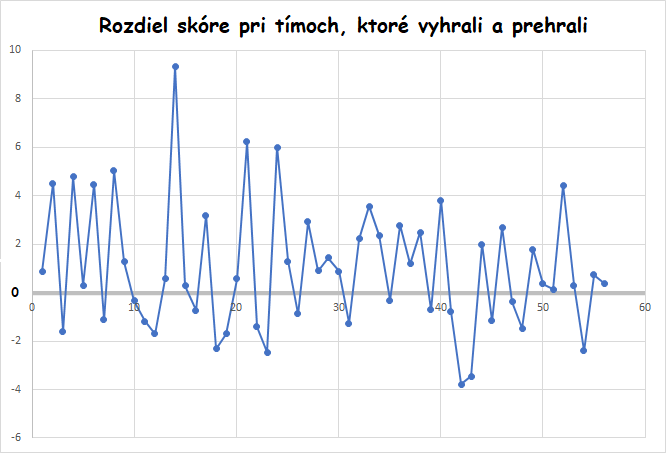
\includegraphics[width=.9\textwidth]{figures/rozdiel}
	\centering
	\caption{ Rozdiel pridaných skóre pri tímoch \label{rozdiel}}
	
\end{figure}

\subsubsection{Známkovanie testovaných tímov}
Pri určovaní známok sme použili tabuľku, o ktorej sme rozprávali v minulej časti. 
\\ \\
Ako môžete vidieť na obrázku \ref{win}, výsledky tímov, ktoré vyhrali, mali všetky prípady, kde tím dostal hodnotenie S+, čo boli 4 tímy. Na druhej strane 1 tím, ktorý vyhral, dostal známku F, konkrétne im bolo pridané skóre 47,9589, čo je na hranici medzi F a E, takisto tím, ktorý porazili, bol ohodnotený známkou D, čo nie je až taký veľký rozdiel a je to predvídateľné.
\\
Väčšina víťazných tímov skončila so známkou B a C, pričom 8 tímov dostalo známku S.
\begin{figure}[h!]
	
	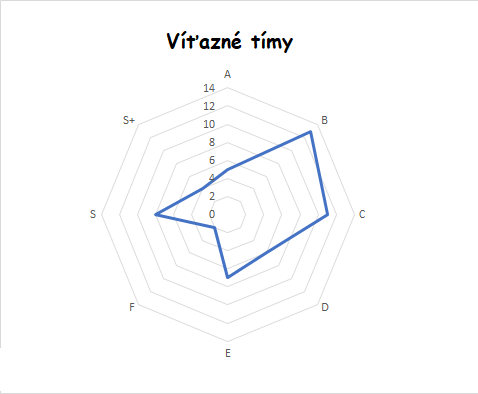
\includegraphics[width=.9\textwidth]{figures/win}
	\centering
	\caption{ Známkovanie víťazných tímov \label{win}}
	
\end{figure}
\\ \\
Na obrázku \ref{lose} vidíme oznámkovanie tímov, ktoré prehrali ich súboj. Najvyššie oznámkovanie bolo S, kde 3 tímy označené druhou najlepšou známkou S prehrali, konkrétne prehrali proti tímom označeným C, B a D. Zhodou okolností súboj tímu S a D bol prípad najväčšieho rozdielu, kde náš model určil nesprávneho víťaza. Rovnako 6 tímov označených známkou A prehralo proti tímom S+, S, S, B, C, D.
\\ 
Najväčšia porcia tímov, ktoré prehrali dostala známku D, C a E, pričom 10 tímov dostalo známku B.

\begin{figure}[h!]
	
	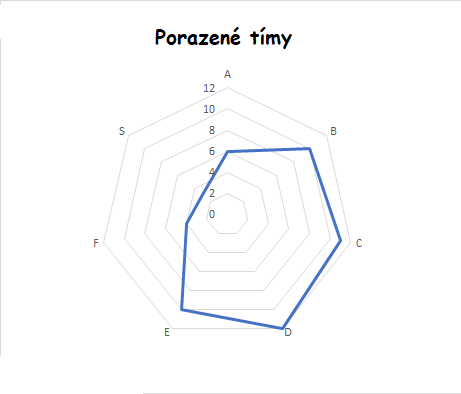
\includegraphics[width=.9\textwidth]{figures/lose}
	\centering
	\caption{ Známkovanie porazených tímov \label{lose}}
	
\end{figure}

\section{Zhodnotenie výsledky testovania}
Výsledky sú lepšie, než sme predpokladali. Je značný rozdiel v tímových kompozíciach, ktorý náš program vie rozoznať.
\\
V testovacej časti sme odhalili, že v 58 prípadoch bolo 31, kde náš program dal víťaznému tímu lepšiu známku, čo reprezentuje 54 percent zo všetkých prípadov.
V 14 prípadoch dostal lepšiu známku tím, ktorý prehral, čo označuje približne 24 percent z celkových prípadov.
V ostatných 13 prípadoch dostali tímy rovnakú známku, čo je približne 22 percent z prípadov.
\\ 
Čo znamená, že ak budeme tipovať na tímy, ktoré majú rozdielne známkovanie, tak máme približne 68,89 percentnú šancu, že náš program dá lepšiu známku tímu, ktorý zápas vyhrá.
